\documentclass[tikz, preview]{standalone}

\usepackage{amsfonts, amsthm, amssymb, amsmath, stmaryrd, etoolbox}
\usepackage{tikz}
\usetikzlibrary{matrix,arrows}

\begin{document}
\[
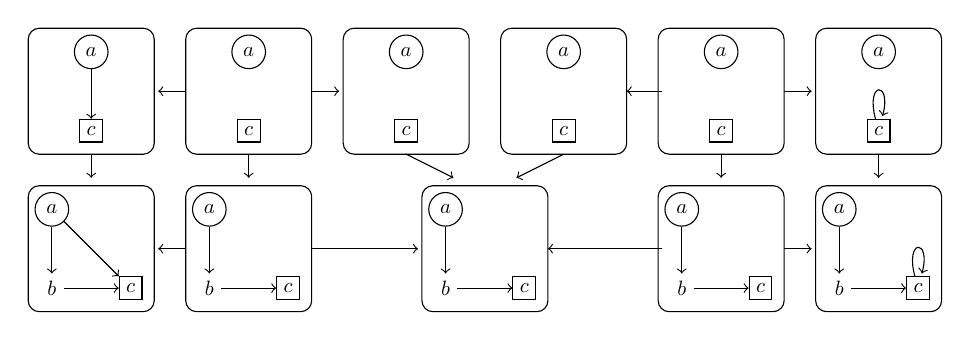
\begin{tikzpicture} 
% TOP ROW BOXES
\draw[rounded corners] (-0.3,1.7) rectangle (1.3,3.3);
\draw[rounded corners] (1.7,1.7) rectangle (3.3,3.3);
\draw[rounded corners] (3.7,1.7) rectangle (5.3,3.3);
\draw[rounded corners] (5.7,1.7) rectangle (7.3,3.3);
\draw[rounded corners] (7.7,1.7) rectangle (9.3,3.3);
\draw[rounded corners] (9.7,1.7) rectangle (11.3,3.3);
% BOTTOM ROW BOXES
\draw[rounded corners] (-0.3,-0.3) rectangle (1.3,1.3);
\draw[rounded corners] (1.7,-0.3) rectangle (3.3,1.3);
\draw[rounded corners] (4.7,-0.3) rectangle (6.3,1.3);
\draw[rounded corners] (7.7,-0.3) rectangle (9.3,1.3);
\draw[rounded corners] (9.7,-0.3) rectangle (11.3,1.3);
% TOP ROW GRAPHS
\node[draw,circle,scale=0.75] (a1) at (0.5,3) {$a$};
\node[draw,rectangle,scale=0.75] (c1) at (0.5,2) {$c$};
\node[draw,circle,scale=0.75] (a2) at (2.5,3) {$a$};
\node[draw,rectangle,scale=0.75] (c2) at (2.5,2) {$c$};
\node[draw,circle,scale=0.75] (a3) at (4.5,3) {$a$};
\node[draw,rectangle,scale=0.75] (c3) at (4.5,2) {$c$};
\node[draw,circle,scale=0.75] (a4) at (6.5,3) {$a$};
\node[draw,rectangle,scale=0.75] (c4) at (6.5,2) {$c$};
\node[draw,circle,scale=0.75] (a5) at (8.5,3) {$a$};
\node[draw,rectangle,scale=0.75] (c5) at (8.5,2) {$c$};
\node[draw,circle,scale=0.75] (a6) at (10.5,3) {$a$};
\node[draw,rectangle,scale=0.75] (c6) at (10.5,2) {$c$};
% BOTTOM ROW GRAPHS
\node[draw,circle,scale=0.75] (a7) at (0,1) {$a$};
\node[scale=0.75] (b1) at (0,0) {$b$};
\node[draw,rectangle,scale=0.75] (c7) at (1,0) {$c$};
\node[draw,circle,scale=0.75] (a8) at (2,1) {$a$};
\node[scale=0.75] (b2) at (2,0) {$b$};
\node[draw,rectangle,scale=0.75] (c8) at (3,0) {$c$};
\node[draw,circle,scale=0.75] (a9) at (5,1) {$a$};
\node[scale=0.75] (b3) at (5,0) {$b$};
\node[draw,rectangle,scale=0.75] (c9) at (6,0) {$c$};
\node[draw,circle,scale=0.75] (a10) at (8,1) {$a$};
\node[scale=0.75] (b4) at (8,0) {$b$};
\node[draw,rectangle,scale=0.75] (c10) at (9,0) {$c$};
\node[draw,circle,scale=0.75] (a11) at (10,1) {$a$};
\node[scale=0.75] (b5) at (10,0) {$b$};
\node[draw,rectangle,scale=0.75] (c11) at (11,0) {$c$};
% GRAPH EDGES
\draw [->] (a1) -- (c1);
\draw (c6) edge [loop above] (c6);
\draw [->] (a7) -- (b1);
\draw [->] (b1) -- (c7);
\draw [->] (a8) -- (b2);
\draw [->] (b2) -- (c8);
\draw [->] (a9) -- (b3);
\draw [->] (b3) -- (c9);
\draw [->] (a10) -- (b4);
\draw [->] (b4) -- (c10);
\draw [->] (a11) -- (b5);
\draw [->] (a7) -- (c7);
\draw [->] (b5) -- (c11);
\draw (c11) edge [loop above] (c11);
% BETWEEN BOX EDGES
\draw [->] (1.7,2.5) -- (1.35,2.5);
\draw [->] (3.3,2.5) -- (3.65,2.5);
\draw [->] (7.75,2.5) -- (7.3,2.5);
\draw [->] (9.3,2.5) -- (9.65,2.5);
\draw [->] (1.7,0.5) -- (1.35,0.5);
\draw [->] (3.3,0.5) -- (4.65,0.5);
\draw [->] (7.75,0.5) -- (6.3,0.5);
\draw [->] (9.3,0.5) -- (9.65,0.5);
\draw [->] (0.5,1.7) -- (0.5,1.4);
\draw [->] (2.5,1.7) -- (2.5,1.4);
\draw [->] (4.5,1.7) -- (5.1,1.4);
\draw [->] (6.5,1.7) -- (5.9,1.4);
\draw [->] (8.5,1.7) -- (8.5,1.4);
\draw [->] (10.5,1.7) -- (10.5,1.4);
\end{tikzpicture}
\]
\end{document}
